La terza sezione di consultazione dei dati raccolti è quella relativa alle detection (cfr. sezione \ref{dati-raccolti}).

\begin{figure}[H]
    \begin{center}
    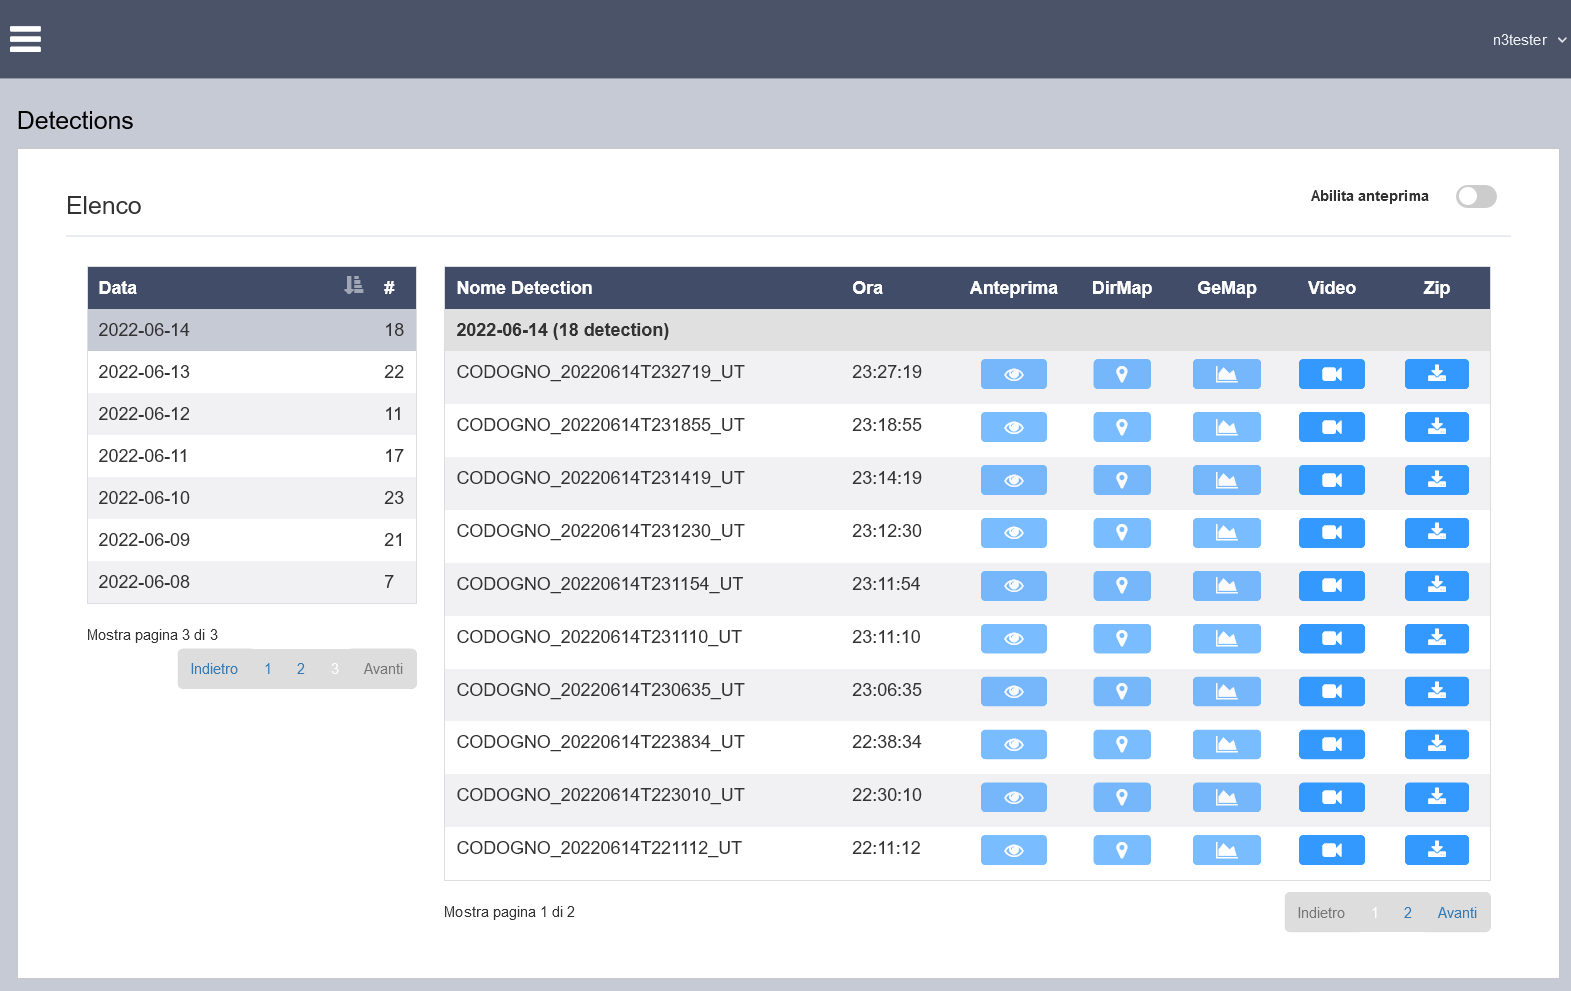
\includegraphics[width=\textwidth]{images/full-detection.png}
    \caption{Sezione \emph{Detection}.}
    \label{fig:detection}
    \end{center}
\end{figure}

\subsection{Visualizzazione dati raccolti} \label{detec-tables}

I dati sono articolati in una doppia tabella analoga a quella delle sezioni \emph{Capture} e \emph{Stack} (cfr. sezione \ref{capture-struct}). Per ogni giorno la seconda tabella mostra l'elenco delle \emph{detection} rilevate, con il nome della cartella, l'ora di rilevazione e cinque pulsanti di interazione: \textbf{Anteprima}, \textbf{DirMap}, \textbf{GeMap}, \textbf{Video} e \textbf{Zip}. È inoltre visibile l'immagine dell'ultima detection rilevata.

\begin{wrapfigure}{r}{0.3\textwidth}
    \vspace{-30pt}
    
\includegraphics[width=0.3\textwidth]{images/toggle-button.jpg}
    \vspace{-30pt}
\end{wrapfigure}
I pulsanti \textbf{Anteprima}, \textbf{DirMap} e \textbf{GeMap} si comportano in modo analogo a quello delle sezioni \emph{Capture} e \emph{Stack}, attivabili dal \textbf{\emph{toggle button}} \emph{Abilita anteprima}. Se cliccati, mostrano in una finestra modale il frame principale della rilevazione convertito in PNG (\emph{Anteprima}) e le immagini BMP DirMap e GeMap (cfr. sezione \ref{dati-raccolti}). Anche in questo caso, la conversione lato server delle immagini di anteprima risulterà in un'attesa di qualche secondo da parte dell'utente.

\begin{figure}[H]
    \begin{center}
    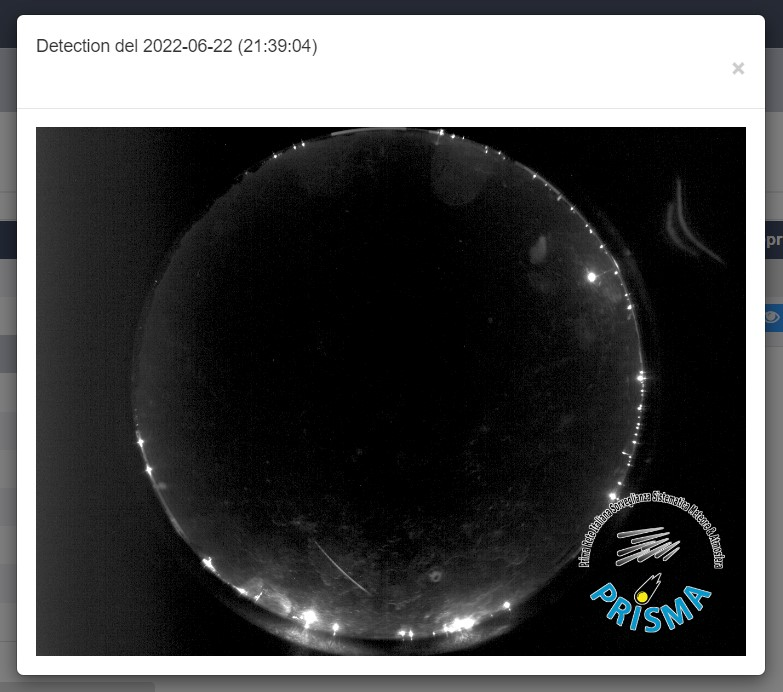
\includegraphics[width=\textwidth]{images/detec-preview.jpg}
    \caption{Anteprima della detection del 22/06/2022.}
    \end{center}
\end{figure}

Cliccando il pulsante \textbf{Video} viene invece scaricato il video della detection, mentre il pulsante \textbf{Zip} richiede lo zip della cartella della detection con i file in essa contenuti. Siccome il processo di elaborazione dei video e degli zip lato server è molto lungo (cfr. sezione \ref{elaborazione-dati-detec}), le richieste sono asincrone e compare un messaggio che avvisa l'utente di attendere qualche minuto prima che avvenga il download.

Inoltre, sempre per il motivo sopracitato, l'utente ha la facoltà di interrompere l'elaborazione in corso cliccando su un pulsante ad hoc (cfr. figure \ref{stop-video} e \ref{stop-zip}) che manda al server una richiesta per interrompere tutti i processi in esecuzione e abortire la chiamata AJAX in modo tale che il client non aspetti la risposta.

Infine, durante la preparazione dello zip o del video vengono disabilitati tutti gli altri pulsanti per ottenere zip o video in modo da non appesantire il server.

\begin{figure}[H]
    \begin{center}
    
\includegraphics[width=\textwidth]{images/stop-video.jpg}
    \caption{Il pulsante rosso permette l'interruzione dell'elaborazione del video sul server.}
    \label{stop-video}
    \end{center}
\end{figure}
\vspace{-24pt}
\begin{figure}[H]
    \begin{center}
    
\includegraphics[width=\textwidth]{images/stop-zip.jpg}
    \caption{Il pulsante rosso permette l'interruzione dell'elaborazione dello zip sul server.}
    \label{stop-zip}
    \end{center}
\end{figure}

\subsection{Elaborazione dei dati server-side} \label{elaborazione-dati-detec}

La consultazione dei dati relativi alle detection impiega consistenti risorse sul server: è stato dunque necessario gestire il più efficientemente possibile l'elaborazione dei dati e i processi ad essi relativi.

\subsubsection{Elaborazione immagini}

L'elaborazione dell'immagine di \textbf{anteprima} corrisponde a quella effettuata con capture e stack, con la conversione in PNG, il watermarking e la codifica in \emph{Base64} (cfr. sezione \ref{elaborazione-dati-capture}).

Le immagini \textbf{DirMap} e \textbf{GeMap} vengono semplicemente codificate in \emph{Base64} e inviate al client.

\subsubsection{Elaborazione video}

La generazione del video attraversa i seguenti stadi:
\begin{enumerate}
    \item \textbf{Conversione dei frame da FITS a PNG}: vengono convertiti tutti i frame formato FITS che individuano la rilevazione in formato PNG con il software \textbf{fitspng} (cfr. sezione \ref{software});
    \begin{verbatim}
        fitspng -o <output_file> <input_file>
    \end{verbatim}
    \item \textbf{Creazione del video}: i frame ottenuti al passo precedente vengono concatenati grazie al software FFmpeg (cfr. sezione \ref{software}), generando il video;
    \begin{verbatim}
        cat <frames_directory>*.png | ffmpeg -f image2pipe \
            -i - <output_video>
    \end{verbatim}
    \item \textbf{Watermarking}: viene applicato sul video generato in basso a destra il logo del progetto PRISMA, ancora con l'utilizzo di FFmpeg.
    \begin{verbatim}
        ffmpeg -i <input_video> -i <logo> -filter_complex \
            'overlay=W-w-5:H-h-5' <output_video>
    \end{verbatim}
\end{enumerate}

L'elaborazione dei video produce due tipi di file temporanei:
\begin{itemize}[noitemsep,nolistsep]
    \item I fotogrammi convertiti in formato PNG
    \item Il video generato senza watermark
\end{itemize}
Tutti questi file sono salvati temporaneamente in una cartella nella webroot e vengono poi cancellati al termine del processo.

\subsubsection{Elaborazione zip}

Viene prodotto lo zip della cartella della detection con tutti i suoi file attraverso il software \textbf{libzip} (cfr. sezione \ref{software}).\\

Dal momento che l'elaborazione dei video e degli zip è problematica in termini di risorse per il nodo, per non appesantire il server e garantire una migliore esperienza all'utente sono state introdotte le seguenti \textbf{tassonomie}:

\begin{shaded}
    \vspace{-12pt}
    \paragraph{Tassonomia 1.}
    \emph{I video (o gli zip) generati vengono mantenuti in memoria fino a quando l'utente decide di liberare lo spazio (cfr. sezione \ref{clean-media}): in questo modo se viene richiesto un video (o uno zip) già generato non se ne deve attendere l'elaborazione. La gestione dello spazio sul nodo di questi media provvisori è dunque demandata all'utente.}
    \paragraph{Tassonomia 2.}
    \emph{Non è possibile richiedere che venga elaborato più di un video (o zip) alla volta.}
    \paragraph{Tassonomia 3.}
    \emph{L'utente ha la possibilità di interrompere la preparazione del video (o zip) in corso, senza aspettare che questa finisca. In questo caso, il server si occupa di fermare tutti i processi in corso inerenti all'elaborazione e pulire i file temporanei.}
\end{shaded}

\begin{figure}[H]
    \begin{subfigure}{\textwidth}
        \begin{center}
        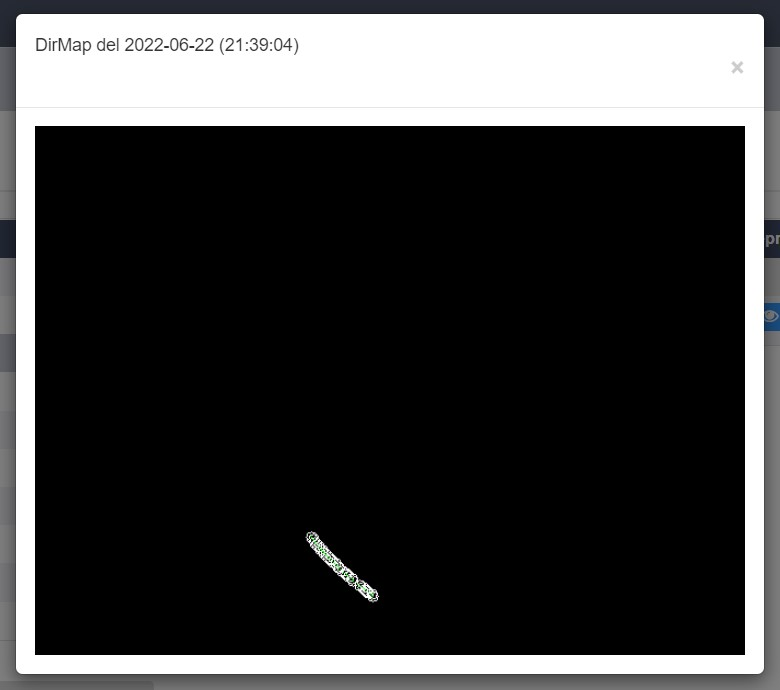
\includegraphics[width=0.85\textwidth]{images/dirmap.jpg}
        \end{center}
    \end{subfigure}
    \begin{subfigure}{\textwidth}
        \begin{center}
        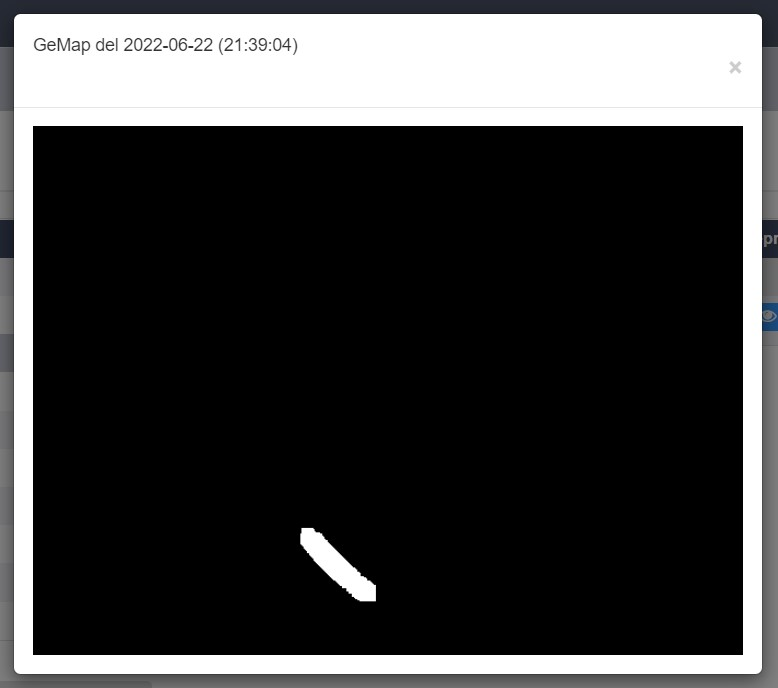
\includegraphics[width=0.85\textwidth]{images/gemap.jpg}
        \end{center}
    \end{subfigure}
    \caption{DirMap e GeMap della detection del 22/06/2022.}
\end{figure}


